%
% quotient1.tex -- Vektorraumquotient
%
% (c) 2021 Prof Dr Andreas Müller, OST Ostschweizer Fachhochschule
%
\documentclass[tikz]{standalone}
\usepackage{amsmath}
\usepackage{times}
\usepackage{txfonts}
\usepackage{pgfplots}
\usepackage{csvsimple}
\usetikzlibrary{arrows,intersections,math}
\begin{document}
\definecolor{darkgreen}{rgb}{0,0.6,0}
\definecolor{darkred}{rgb}{0.7,0,0}
\def\skala{1}
\begin{tikzpicture}[>=latex,thick,scale=\skala]

\node at (0,0) {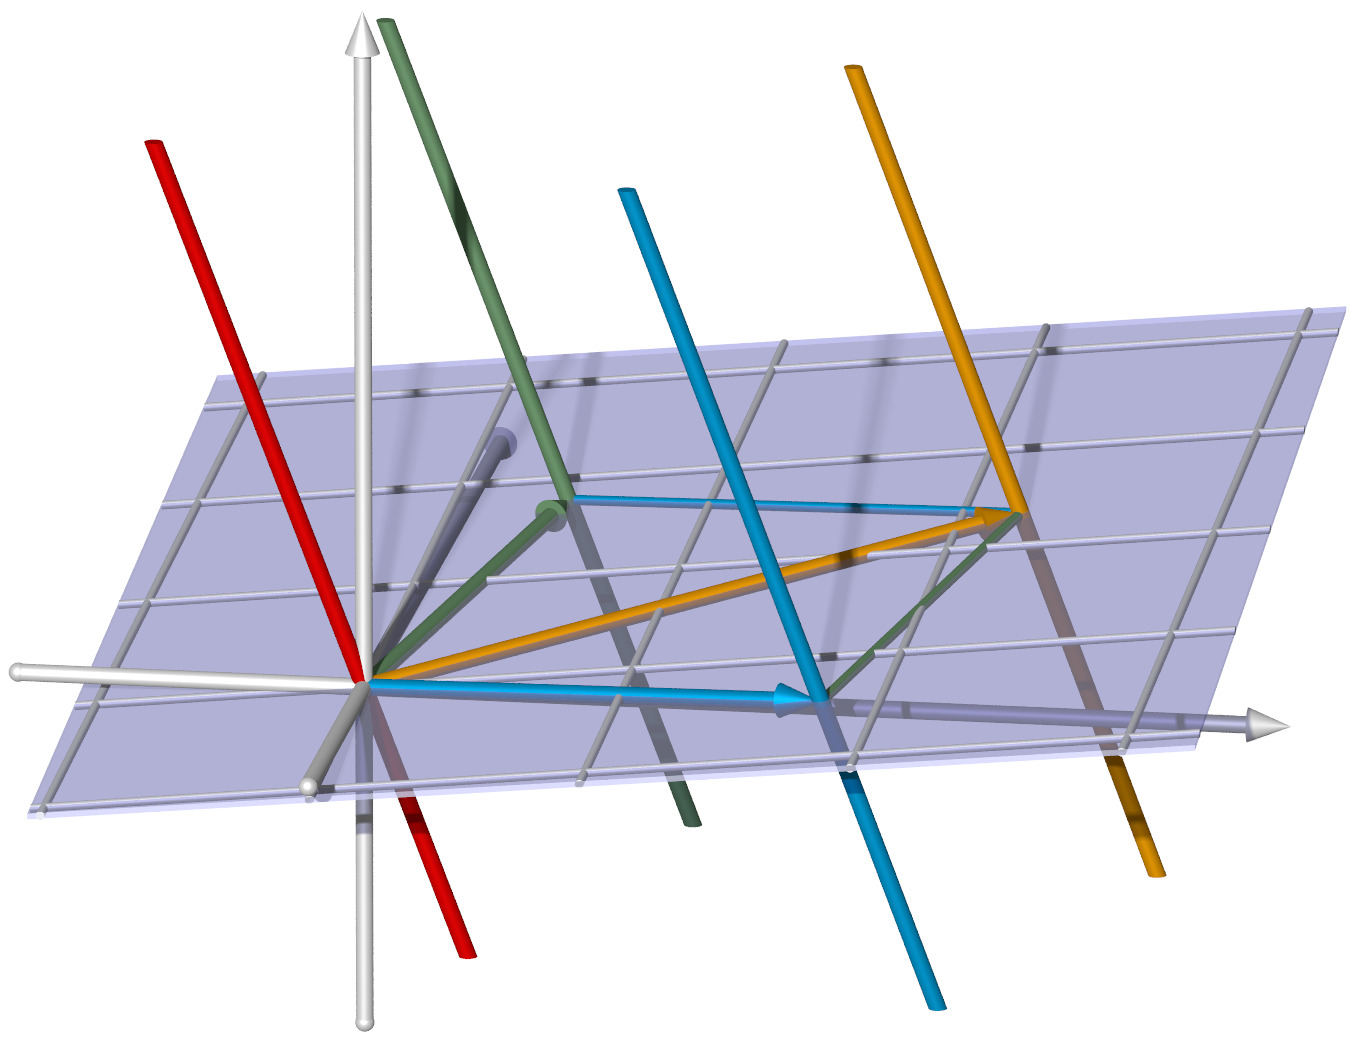
\includegraphics[width=8cm]{quotient1.jpg}};

\node[color=blue] at (0.7,-1.3) {$v$};
\node[color=darkgreen] at (-1.0,0.1) {$w$};
\node[color=orange] at (2.5,0.1) {$v+w$};
\node[color=darkred] at (-2.1,-0.9) {$0$};
\node[color=darkred] at (-3.1,2.4) {$U$};

\end{tikzpicture}
\end{document}

